\documentclass{minimal}
\usepackage{pgf}
\usepackage{tikz}
\usepackage[utf8]{inputenc}
\usetikzlibrary{arrows,automata}
\usetikzlibrary{positioning}
\usetikzlibrary{fit}
\usetikzlibrary{calc}

\tikzset{
  state/.style={
    rectangle,
    rounded corners=1pt,
    draw=black, very thick,
    minimum height=2em,
    inner sep=2pt,
    text centered,
  },
}


\begin{document}
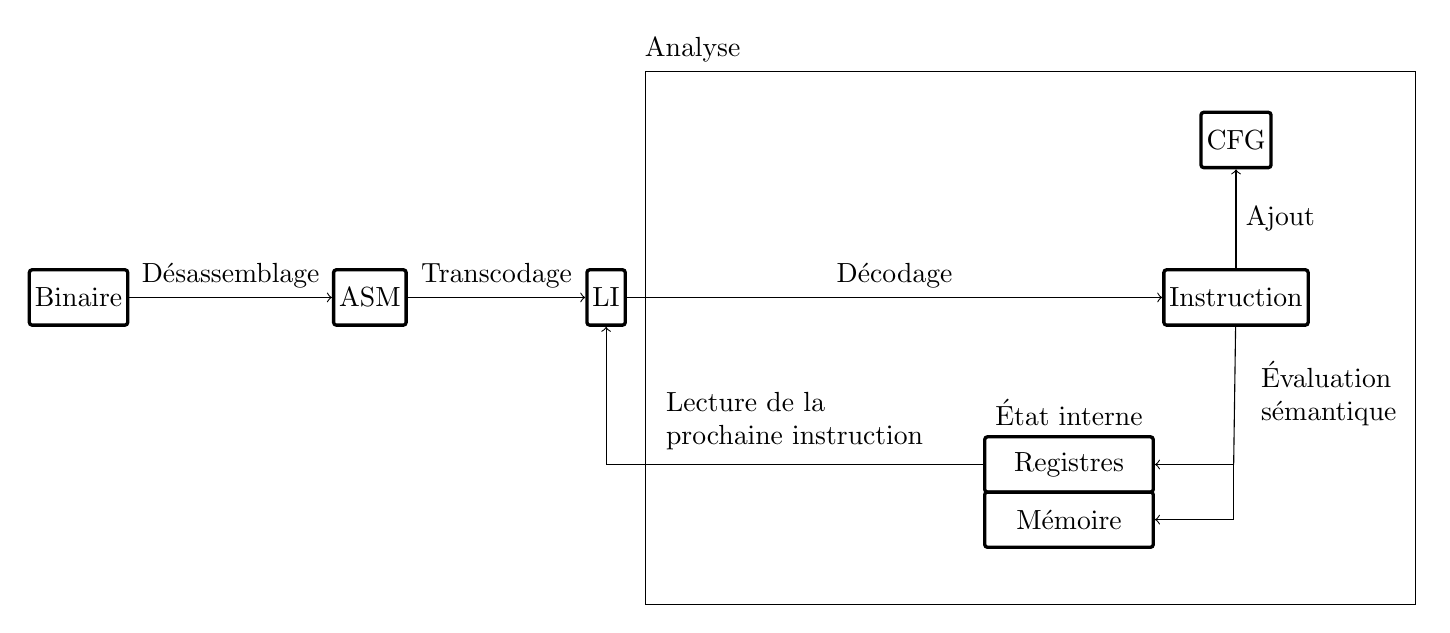
\begin{tikzpicture}[->]

\node[state] (BIN){
  Binaire
};

\node[state,
  right of=BIN,
  node distance=3.7cm,
  anchor=center] (ASM)
  {
    ASM
  };

\node[state,
  right of=ASM,
  node distance=3.0cm,
  anchor=center]
  (IR){
    LI
  };

\node[state,
    anchor=center,
    right of=IR,
    node distance=8cm
    ]
    (INST){
      Instruction
    };
    
\node[state,
    anchor=center,
    above of=INST,
    node distance=2cm
    ]
    (CFG){
      CFG
    };

\node[state,
    label=État interne,
    anchor=center,
    below left of=INST,
    text width=2cm,
    node distance=3cm
    ]
    (ETAT_REG){
      Registres
    };

\node[state,
    anchor=center,
    below of=ETAT_REG,
    text width=2cm,
    node distance=0.7cm
    ]
    (ETAT_MEM){
      Mémoire
    };

\coordinate [right=1cm of ETAT_REG] (hub1) {};
\coordinate [right=1cm of ETAT_MEM] (hub2) {};
\coordinate (hub3) at ($ (hub1)!(IR.south)!(ETAT_REG.east) $);
\coordinate [above=2.5cm of IR.north] (ABIR) {};
\coordinate [right=0.5cm of ABIR] (coin1);
\coordinate [below=0.7cm of ETAT_MEM.south] (b);
\coordinate [right=4.4cm of b] (coin2);
\coordinate [right=0.6cm of coin1] (l);
\node[above] at (l) {Analyse};
\draw[label=aa] (coin1) rectangle(coin2);

\path
  (BIN) 	  edge    node[anchor=south,above]{Désassemblage}           (ASM)
  (ASM)     edge    node[anchor=south,above]{Transcodage}             (IR)
  (IR)      edge    node[anchor=south,above]{Décodage}                (INST)
  (INST)    edge    node[anchor=south,right]{Ajout}                   (CFG)
  
  (INST)    edge[-]   
    node[anchor=south,right]{
    \begin{tabular}{l}
      Évaluation\\
      sémantique
    \end{tabular}}             (hub1)
    
  (hub1)    edge[-] node[anchor=south,right]{}                       (hub2)
  (hub1)    edge    node[anchor=east,above]{}                        (ETAT_REG.east)
  (hub2)    edge    node[anchor=right,above]{}                       (ETAT_MEM.east)
  
  (ETAT_REG.west)    edge[-]   
    node[anchor=west, above]{
      \begin{tabular}{l}
        Lecture de la\\
        prochaine instruction               
      \end{tabular} }
      (hub3)
      
  (hub3)    edge    node[anchor=south,below]{}                       (IR.south)
;

\end{tikzpicture}
\end{document}
